\documentclass[12pt]{article}

\usepackage[utf8]{inputenc}
\usepackage[letterpaper, includefoot, margin=0.5in]{geometry}
\usepackage{multicol}
\usepackage{datetime}
\usepackage{fancyhdr}
\usepackage[table]{xcolor}
\usepackage{bbding}
\usepackage{fontawesome}
\usepackage{multirow}
\usepackage{graphicx}
\usepackage{longtable}
\usepackage{hyperref}
\usepackage{verbatim}
\usepackage{wrapfig}
\usepackage{supertabular,booktabs}
\usepackage{scrextend}
\usepackage{indentfirst}
\usepackage{CJKutf8}
\usepackage{textcomp}
\usepackage[font=small, labelfont=bf]{caption}
\usepackage{savetrees}
\usepackage{fdsymbol}
\usepackage{enumitem}
\usepackage{tikz}
\usetikzlibrary{shapes,arrows}
\usepackage[scaled]{CountriesOfEurope}
%\usepackage{titlesec}
%\usepackage{marvosym}

\newcolumntype{y}[1]{>{\raggedright\let\newline\\\arraybackslash\hspace{0pt}}m{#1}}
\newcolumntype{x}[1]{>{\centering\let\newline\\\arraybackslash\hspace{0pt}}m{#1}}
\newcolumntype{z}[1]{>{\raggedleft\let\newline\\\arraybackslash\hspace{0pt}}m{#1}}

\setlength{\parindent}{5mm}

\newdateformat{mydate}{\dayofweekname{\the\day}{\the\month}{\the\year}, \monthname[\the\month] \the\day, \the\year}

\pagestyle{fancy}
\fancyhf{}
\lfoot{\copyright Spadyal 2018--\the\year}
\cfoot{\thepage}
\rfoot{\mydate\today}
\renewcommand{\headrulewidth}{0pt}

\renewcommand*\contentsname{Table of Contents}

\title{GDD}

%-------------------------%
%--Story Code / Startup---%
%-------------------------%
\newcommand{\thought}[1]{\textit{#1}}

\newcommand{\scenechange}{
\par
\vspace{\baselineskip}
\par
\noindent}
%Creates a line break for a change of scene

\newcommand{\majorchange}{
\par
\vspace{\baselineskip}
\hfill
\textasteriskcentered
\hfill
\vspace{\baselineskip}
\noindent}
%creates a major line break, split by an asterisk for scene changes at the end of a page of where a sense of a major change is required. 

\makeatletter
\renewcommand\@biblabel[1]{}
\makeatother
%Removes labels of each reference in the bibliography

\begin{comment}
\titleclass{\subsubsubsection}{straight}[\subsection]

\newcounter{subsubsubsection}[subsubsection]
\renewcommand\thesubsubsubsection{\thesubsubsection.\arabic{subsubsubsection}}
\renewcommand\theparagraph{\thesubsubsubsection.\arabic{paragraph}} % optional; useful if paragraphs are to be numbered

\titleformat{\subsubsubsection}
{\normalfont\normalsize\bfseries}{\thesubsubsubsection}{1em}{}
\titlespacing*{\subsubsubsection}
{0pt}{3.25ex plus 1ex minus .2ex}{1.5ex plus .2ex}
%Creates a new level of a section
\end{comment}

\tikzstyle{decision} = [diamond, draw, fill=blue!20, 
text width=4.5em, text badly centered, node distance=2.5cm, inner sep=0pt] %node distance=3cm
\tikzstyle{block} = [rectangle, draw, fill=blue!20, 
text width=5em, text centered, rounded corners, minimum height=4em]
\tikzstyle{line} = [draw, -latex']
\tikzstyle{cloud} = [draw, ellipse,fill=red!20, node distance=3cm,
minimum height=2em]

\begin{document}

\begin{titlepage}
\centering
[insert box cover here]
%\includegraphics[width=in]{}
\end{titlepage}

\clearpage
\setcounter{page}{2}

\begin{center}
%\includegraphics[width=4in]{} \\
\vspace{0.15in}
\hrule
\vspace{0.15in}
\textbf{Title} \par
\vspace{0.15in}
Document Version 0.1.5 \par
\end{center}
\textbf{Written by Spadyal} \newline \newline
Bryant Benzant \newline \newline
bryantbenzant@gmail.com $\bullet$ (914) 826-7716 \newline \newline
Compiled with \LaTeX
\newpage

\twocolumn
\tableofcontents
\newpage

\twocolumn
\section{Revision History}
\noindent Version 0.1.0 -– Monday, October 8, 2018
\begin{addmargin}[5mm]{0em}
Document Format
\end{addmargin}
\noindent Version 0.1.1 -– Saturday, October 13, 2018
\begin{addmargin}[5mm]{0em}
Game Goals, Game Levels Format
\end{addmargin}
\noindent Version 0.1.2 -– Tuesday, November 13, 2018
\begin{addmargin}[5mm]{0em}
Game Goals, Story Overview, Game Controls, Technological Requirements, Front End of the Game, Title/Start Screen, Game Flowchart, Player Inventory Tools, Power-Ups, Rewards \& Economy, Health, World Overview, Universal Game Mechanics, Game Levels, Marketing Plan
\end{addmargin}
\noindent Version 0.1.3 -– Wednesday, November 14, 2018
\begin{addmargin}[5mm]{0em}
Game Flowchart, Power-Ups
\end{addmargin}
\noindent Version 0.1.4 -– Thursday, November 15, 2018
\begin{addmargin}[5mm]{0em}
Game Levels Format Extended
\end{addmargin}
\noindent Version 0.1.5 -– Tuesday, November 27, 2018
\begin{addmargin}[5mm]{0em}
Game Goals, Game Levels
\end{addmargin}
%\noindent Version 0.1.6 -– Tuesday, November 20, 2018
\begin{addmargin}[5mm]{0em}

\end{addmargin}
\onecolumn

\section{Game Goals}
\subsection*{``Back of the box'' Goals}
\begin{addmargin}[5mm]{0em}
\begin{itemize}[noitemsep]
\item Shop and purchase products from real-world brands to fight enemies and explore new worlds
%\item Play multiplayer (locally) with up to 4 characters
\item Talk to people to help you out during your adventure
\end{itemize}
\end{addmargin}
\subsection*{High Concept}
\noindent \textbf{Title} is an action-adventure and open world platformer that lets the player choose a character---up to four players can choose any of the eight characters---and plays a world where they have to go around some levels to find stores and buy specific items that are required for completing other levels. \newline \newline
This game has a hybrid of genres including:
\begin{addmargin}[10mm]{0em}
\begin{itemize}[noitemsep]
\item Sandbox (Open World)
\item Platformer
%\item Adventure
\item Rhythm
%\item Shooter
%\item Strategy
\end{itemize}
\end{addmargin}
More information about what these genres do for the game will be discussed shortly.
\subsection*{Who, What, How?}
\begin{addmargin}[5mm]{0em}
\begin{itemize}[noitemsep]
\item \textbf{Who:} This game is directed towards teens, or ages 12 and up (Rating: T for Teen).
\item \textbf{What:} 
\item \textbf{How:} 
\end{itemize}
\end{addmargin}
\subsection*{Platform}
PC \& Mac (iOS \& Android [as a native app] is a possibility)
\subsection*{Descriptions of Gameplay Types}
\begin{addmargin}[5mm]{0em}
\begin{itemize}[noitemsep]
\item \textbf{Sandbox (Open World)} = Each world has an open-ended inside and outside map (hub worlds) on four areas--each stage is connected to two hub worlds. Those hub worlds are: (1) the city (including the airport and the mall), (2) the academia, and (3) the residential area. Each of those hub worlds is where the player can talk to NPC's and buy products.
\item \textbf{Platformer} = The stages that connect to hub worlds are basically platformer levels where the player can run, jump, fight, drive, etc.
%\item \textbf{Adventure} = 
%\item \textbf{Rhythm} = %There is a stage on page \iffalse \pageref{} \fi that lets the player move from one place to another, but requires hand-eye coordination on a rhythm-based minigame.
\end{itemize}
\end{addmargin}
\newpage

\begin{comment}
\section{Story Overview}
%\section*{\underline{Version 1}}
\begin{multicols}{2}
\subsection*{Prelude}
\noindent 
\subsection*{Chapter 1: Route 6}
\noindent 
\subsection*{Chapter 2: Candy Country}
\noindent 
\subsection*{Chapter 3: Aqua Beach}
\noindent 
\subsection*{Chapter 4: Winter Paradise}
\noindent 
\subsection*{Chapter 5: Vernal Forest}
\noindent 
\subsection*{Chapter 6: Game Network}
\noindent 
\subsection*{Chapter 7: Astral Sky}
\noindent 
\subsection*{Chapter 8: Base Code 255}
\noindent 
\subsection*{Ending}
\noindent
\end{multicols}
\newpage
\end{comment}

\section{Licensor Points \& Concerns}
\begin{center}
\tablehead{
\textbf{Person} & \textbf{Title} & \parbox[c]{1.75in}{\textbf{Social Network Links}} \\}

\tablelasttail{
\\
}

\begin{supertabular}{c|x{2in}|x{1.75in}}
\hline
Spadyal & Game Design, Level Design, Art, Programming, Writing & \href{http://staream.deviantart.com/}{
\includegraphics[width=0.2in]{deviantart}}\href{https://www.facebook.com/spadyalofficial/}{
\includegraphics[width=0.2in]{facebook}}\href{}{
\includegraphics[width=0.2in]{instagram}}\href{https://soundcloud.com/spadyalofficial}{
\includegraphics[width=0.2in]{soundcloud}}\href{}{
\includegraphics[width=0.2in]{tumblr}}\href{https://twitter.com/Spadyal1}{
\includegraphics[width=0.2in]{twitter}}\href{}{
\includegraphics[width=0.2in]{www}}\href{}{
\includegraphics[width=0.2in]{youtube}} \\ \hline
Scott Rogers & Special Thanks & \href{https://twitter.com/mightybedbug?ref_src=twsrc\%5Egoogle\%7Ctwcamp\%5Eserp\%7Ctwgr\%5Eauthor}{
\includegraphics[width=0.2in]{twitter}} %\\ \hline
%SOUNDSCVPE & Music & \href{https://www.facebook.com/Soundcvpe-214495038749477/}{
\includegraphics[width=0.1in]{facebook}}\href{https://soundcloud.com/soundscvpe-mewsic}{
\includegraphics[width=0.1in]{soundcloud}}\href{https://twitter.com/SOUNDSCVPE}{
\includegraphics[width=0.1in]{twitter}}\href{https://www.youtube.com/channel/UCtR18SFn3YqcU98oVHOhzKw}{
\includegraphics[width=0.1in]{youtube}} \\ \hline
%iMeiden & Music & \href{https://soundcloud.com/meiden}{
\includegraphics[width=0.1in]{soundcloud}}\href{https://twitter.com/itosyunn}{
\includegraphics[width=0.1in]{twitter}} \\ \hline
%Miruku & Music & \href{https://www.facebook.com/mirukumusic}{
\includegraphics[width=0.1in]{facebook}}\href{https://www.instagram.com/mirukumusic/}{
\includegraphics[width=0.1in]{instagram}}\href{https://soundcloud.com/mirukumusic}{
\includegraphics[width=0.1in]{soundcloud}}\href{https://www.youtube.com/channel/UCHZZFExyVSWR1gAj0nwye6g}{
\includegraphics[width=0.1in]{youtube}} \\ \hline
%Firefly Music & Special Thanks & \href{https://www.facebook.com/FireflyAMV}{
\includegraphics[width=0.1in]{facebook}}\href{https://soundcloud.com/fireflyamv}{
\includegraphics[width=0.1in]{soundcloud}}\href{https://twitter.com/FireflyAMV}{
\includegraphics[width=0.1in]{twitter}}\href{https://www.youtube.com/user/fireflies2781996/featured}{
\includegraphics[width=0.1in]{youtube}} \\ \hline
%Ebon & Music & \href{}{
\includegraphics[width=0.1in]{facebook}}\href{}{
\includegraphics[width=0.1in]{instagram}}\href{}{
\includegraphics[width=0.1in]{soundcloud}}\href{}{
\includegraphics[width=0.1in]{twitter}}\href{}{
\includegraphics[width=0.1in]{www}} \\ \hline
%Snail's House & Music & \href{}{
\includegraphics[width=0.1in]{facebook}}\href{}{
\includegraphics[width=0.1in]{instagram}}\href{}{
\includegraphics[width=0.1in]{soundcloud}}\href{}{
\includegraphics[width=0.1in]{twitter}}\href{}{
\includegraphics[width=0.1in]{www}} \\ \hline
%Harito & Music & \href{}{
\includegraphics[width=0.1in]{facebook}}\href{}{
\includegraphics[width=0.1in]{instagram}}\href{}{
\includegraphics[width=0.1in]{soundcloud}}\href{}{
\includegraphics[width=0.1in]{twitter}}\href{}{
\includegraphics[width=0.1in]{www}} \\ \hline
%OHEY & Music & \href{}{
\includegraphics[width=0.1in]{facebook}}\href{}{
\includegraphics[width=0.1in]{instagram}}\href{}{
\includegraphics[width=0.1in]{soundcloud}}\href{}{
\includegraphics[width=0.1in]{twitter}}\href{}{
\includegraphics[width=0.1in]{www}} \\ \hline
%KOTONOHOUSE & Music & \href{}{
\includegraphics[width=0.1in]{facebook}}\href{}{
\includegraphics[width=0.1in]{instagram}}\href{}{
\includegraphics[width=0.1in]{soundcloud}}\href{}{
\includegraphics[width=0.1in]{twitter}}\href{}{
\includegraphics[width=0.1in]{www}} \\ \hline
%PIKASONIC & Music & \href{https://soundcloud.com/pika5onic}{
\includegraphics[width=0.1in]{soundcloud}}\href{https://twitter.com/PIKASONIC_ofc}{
\includegraphics[width=0.1in]{twitter}}\href{https://www.youtube.com/channel/UC2ne9XqtBWKJKLfIAKtmjAg}{\includegraphics[width=0.1in]{youtube}} \\ \hline
%Kazmasa & Music & \href{}{\includegraphics[width=0.1in]{facebook}}\href{}{\includegraphics[width=0.1in]{instagram}}\href{}{\includegraphics[width=0.1in]{soundcloud}}\href{}{\includegraphics[width=0.1in]{twitter}}\href{}{\includegraphics[width=0.1in]{www}} \\ \hline
\end{supertabular}
\end{center}

\noindent All credit is given in the game credits and in the website along with social links.
\onecolumn

\section{Game Controls}
\begin{itemize}[noitemsep]
\item Press the arrow keys to walk
\item Press the Z Button to jump
\item Press the X Button to perform an action depending on the level; for example(s):
\begin{itemize}[noitemsep,nosep]
\item attack for \textbf{Fight Level}
\item accelerate for \textbf{Speed Level}
%\item dig for \textbf{Dig Level}
%\item  for \textbf{Stealth Level}
%\item perform an action for \textbf{Puzzle Level}
\end{itemize}
\item Press the A Button to perform a special action
\item Press the S Button to perform a tag (or team) action (if there are at least two players)
\item Press the Backspace Button to pause
\item Press the F6 Button to open the Debug Menu
\end{itemize}
*\textit{Note: The player can customize the controls (both keyboard and gamepad)}
\vfill

\section{Technological Requirements}
\noindent \textbf{Godot Engine} will be used to code the game and make the game art.
\vfill

\begin{comment}
\section{Loading Screen}
\noindent The Loading Screen is shown before the game starts
\begin{center}
%\includegraphics[width=4.45in]{Loading_Screen}
\end{center}
\end{comment}

\section{Front End of the Game}
\begin{center}
\includegraphics[width=2.5in]{Front_End_Of_The_Game}
\end{center}
\vfill

\section{Title/Start Screen}
\noindent After the Spadyal logo, the player is taken to the start screen. The player will have three options: New Game, Continue, Special, and Options. New Game lets the player begin to play the game for the first time. Continue takes the player to a menu where they saved their previous progress on the game. Special shows the player bonus materials and achievements; this option will only show if the player has beaten the game. Options lets players change the settings on the game.
\newpage

\section{Game Flowchart}
\begin{center}
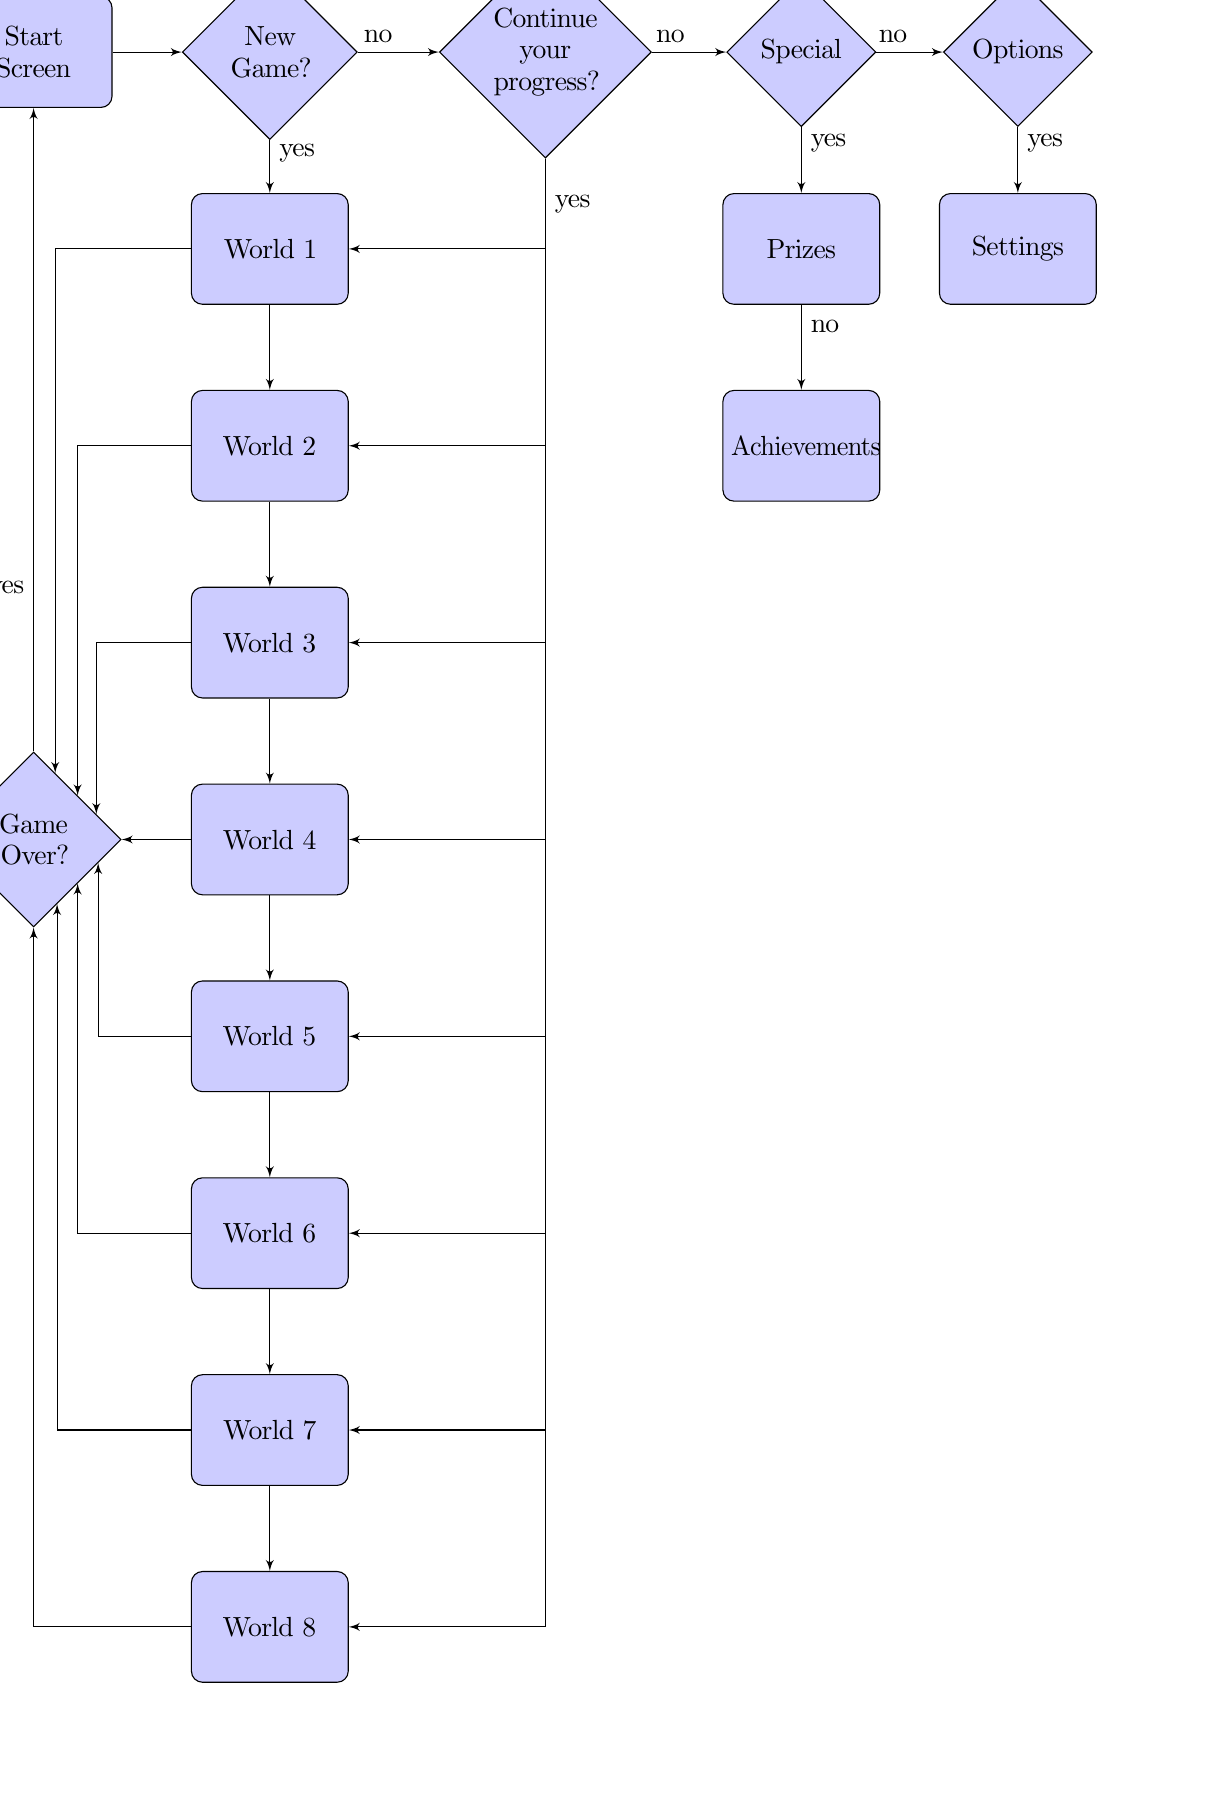
\begin{tikzpicture}[node distance = 2.5cm, auto]
% Place nodes
\node [block] (init) {Start Screen};
\node [decision, right of=init, node distance=3cm] (newgame) {New Game?};
\node [decision, right of=newgame, node distance=3.5cm] (continue) {Continue your progress?};
\node [decision, right of=continue, node distance=3.25cm] (special) {Special};
\node [decision, right of=special, node distance=2.75cm] (options) {Options};
\node [block, below of=newgame] (game1) {World 1};
\node [block, below of=game1] (game2) {World 2};
\node [block, below of=game2] (game3) {World 3};
\node [block, below of=game3] (game4) {World 4};
\node [block, below of=game4] (game5) {World 5};
\node [block, below of=game5] (game6) {World 6};
\node [block, below of=game6] (game7) {World 7};
\node [block, below of=game7] (game8) {World 8};
\node [decision, left of=game4, node distance=3cm] (gameover) {Game Over?};
\node [block, below of=special] (prizes) {Prizes};
\node [block, below of=prizes] (achievements) {Achievements};
\node [block, below of=options] (settings) {Settings};
% Draw edges
\path [line] (init) -- (newgame);
\path [line] (newgame) -- node [near start] {yes} (game1);
\path [line] (newgame) -- node [near start] {no} (continue);
\path [line] (continue) |- node [near start] {yes} (game1);
\path [line] (continue) |- (game2);
\path [line] (continue) |- (game3);
\path [line] (continue) |- (game4);
\path [line] (continue) |- (game5);
\path [line] (continue) |- (game6);
\path [line] (continue) |- (game7);
\path [line] (continue) |- (game8);
\path [line] (continue) -- node [near start] {no} (special);
\path [line] (special) -- node [near start] {no} (options);
\path [line] (game1) -- (game2);
\path [line] (game2) -- (game3);
\path [line] (game3) -- (game4);
\path [line] (game4) -- (game5);
\path [line] (game5) -- (game6);
\path [line] (game6) -- (game7);
\path [line] (game7) -- (game8);
\path [line] (game1) -| (gameover.72.5);
\path [line] (game2) -| (gameover.north east);
\path [line] (game3) -| (gameover.22.5);
\path [line] (game4) -- (gameover);
\path [line] (game5) -| (gameover.340.5);
\path [line] (game6) -| (gameover.south east);
\path [line] (game7) -| (gameover.290.5);
\path [line] (game8) -| (gameover);
\path [line] (gameover) -- node [near start] {yes} (init);
\path [line] (special) -- node [near start] {yes} (prizes);
\path [line] (prizes) -- node [near start] {no} (achievements);
\path [line] (options) -- node [near start] {yes} (settings);
\end{tikzpicture}
\end{center}
\begin{comment}
\twocolumn

\section{Game Camera}


\section{HUD System}
\noindent \textbf{Health}
\begin{addmargin}[5mm]{0em}

\end{addmargin}
\noindent \textbf{Economy}
\begin{addmargin}[5mm]{0em}

\end{addmargin}
\noindent \textbf{Ammunition}
\begin{addmargin}[5mm]{0em}
\indent  \newline
\end{addmargin}
\noindent \textbf{Abilities}
\begin{addmargin}[5mm]{0em}

\end{addmargin}
\noindent \textbf{Options}
\begin{addmargin}[5mm]{0em}

\end{addmargin}
\end{comment}
\newpage

\begin{comment}
\section{Player Characters}
\noindent 
\begin{center}
%\includegraphics[width=2in]{All_Characters}
\end{center}
\end{comment}
\newpage

\section{Player Inventory Tools}
\begin{multicols}{2}
\begin{itemize}[noitemsep]
\item Car Parts
\begin{itemize}[noitemsep,nosep]
\item Battery
\item Brakes \& Traction Control Systems
\item Bumper Accessories
\item Engine
\item Headlamps / Headlights
\item Tires
\item Oil
\item Wheels
\item Exhaust
\item Windshields
\item Covers
\item Sensors
%\item 
\end{itemize}
\item Motorcycle Parts
\begin{itemize}[noitemsep,nosep]
\item Tires
\item Seats
\item Air Intake
\item Lighting
\item Speedometer
\item Exhaust
\end{itemize}
\item Kitchenware
\begin{itemize}[noitemsep,nosep]
\item Spoons
\item Bottle Opener
%\item 
\end{itemize}
\item Summer (Water) Clothing
\item Surf Gear
\begin{itemize}[noitemsep,nosep]
\item Surfboard
%\item 
\end{itemize}
\item Winter Clothing
\item Winter Gear
\begin{itemize}[noitemsep,nosep]
\item Gloves
\item Boots
\item Rollerskates
\end{itemize}
\item Spring (Outdoor) Clothing
\item Outdoor Gear
\begin{itemize}[noitemsep,nosep]
\item Lantern
\item Headlamp/Flashlight
\item Adventure Duffle
\item Multi-tool
\item Firestarter
\item Matches
\item Lighter
\item Carabiner
%\item 
\end{itemize}
\item Electronic Gadgets
\begin{itemize}[noitemsep,nosep]
\item Drone
\item Portable Scanner
\item Keyboard Projector
\item Projector
\end{itemize}
\item Airplane Parts
\item Model Rocket Parts
\end{itemize}
\end{multicols}
\newpage

%\section{Combat}
%\noindent \textbf{}
%\begin{addmargin}[5mm]{0em}

%\end{addmargin}
%\onecolumn
%\newpage

\section{Power-Ups}
\begin{multicols}{2}
\begin{itemize}[noitemsep]
\item Road Trip
\begin{itemize}[noitemsep,nosep]
\item Popcorn
\item Chips
\item French Fries
\item Water
\item Burgers
\item Hot Dogs
\item Steak
\item Fried Chicken
\end{itemize}
\item Sweets
\begin{itemize}[noitemsep,nosep]
\item Cake
\item Gummy Candy
\item Licorice
\item Sour Candy
\item Chocolate
\item Ice Cream
\item Belgian Waffles
\item Doughnuts
\item Fudge
\end{itemize}
\item Summer
\begin{itemize}[noitemsep,nosep]
\item Ramune (\begin{CJK}{UTF8}{min}ラムネ\end{CJK})
\item Cola (\begin{CJK}{UTF8}{min}コーラ\end{CJK})
\item Watermelon
\item Iced Tea (\begin{CJK}{UTF8}{min}アイスティ\end{CJK})
\item Cheesecake
\item Scrambled Eggs
\item Calamari
\item Shrimp
\item Salmon
\end{itemize}
\columnbreak
\item Winter
\begin{itemize}[noitemsep,nosep]
\item Coffee
\item Oatmeal
\item Hot Chocolate
\item Green Tea
\item Gingerbread
\item Eggnog
\item Apple Pie
\item Pumpkin Pie
\item Turkey
\end{itemize}
\item Spring
\begin{itemize}[noitemsep,nosep]
\item Fruits
\item Vegetables
\item Venison Beef Jerky
\item Pizza
\item Garlic Bread
\item Pasta
\item Lasagna
\item Calzone
\item Tiramisu
%\item 
\end{itemize}
\item Asian Food
\begin{itemize}[noitemsep,nosep]
\item Japanese Sushi (\begin{CJK}{UTF8}{min}すし\end{CJK})
\item Japanese Ramen (\begin{CJK}{UTF8}{min}ラーメン\end{CJK})
\item Japanese Curry
\item Chinese Rice
\item Chinese Egg Rolls
\item Chicken
\item Pork
\item Beef
\item Fish
\item Dumplings
\end{itemize}
\end{itemize}
\end{multicols}
\begin{comment}
\noindent \textbf{} \newline
\indent  \newline\newline
\noindent \textbf{} \newline
\indent  \newline\newline
\noindent \textbf{} \newline
\indent  \newline
\indent Cost:  \newline\newline
\noindent \textbf{} \newline
\indent  \newline
\indent Cost:  \newline\newline
\end{comment}
\onecolumn

\section{Rewards \& Economy}
\noindent Since this game is a free download (from the website), the player will be able to collect and spend one currency in the game: \textbf{Dollars (\$)}. %\textbf{Yen (\textyen)}.
\begin{center}
\textbf{\Huge \$}
\end{center}
\subsection{Shops}
\noindent Each Hub World has either a mall, plaza, or a small shopping center where the player can buy tools/equipment, gear, parts, and food. \newline \newline
Each shop can let the player have a shopping cart gathering store items before paying. If the player were to walk out of the store, the items won't be removed from their shopping cart until $(5 < x < 10) \textrm{ where } x$ is the number of minutes in the range has passed; this will be called a ``Clipboard.'' \newline \newline
*\textit{The player's history of purchases will be recorded in a database for an achievement.}
\subsection{Dollars}
\noindent At the beginning of the game, the player earns \textbf{\$}300\iffalse 34,000 \$ ($\approx$ \$302) \fi. \textbf{\$} can be found in the following types of levels:
\begin{description}[align=right,labelwidth=3cm,noitemsep]
\item [Fight Level:] \textbf{\$} can be picked up after defeating an enemy, dropping \textbf{\$} behind
\item [Platform Level:] \textbf{\$} can be picked up in several areas of this type of level, including shortcuts and secret areas
\item [Dig Level:] \textbf{\$} can be found in secret areas underground
\item [Stealth Level:] \textbf{\$} can be found in secret areas of a building, site, etc.
\item [Combo Level:] all of the above
\end{description}
\vfill

\section{Health}
\noindent \textbf{Health} \newline
\indent Health is lost by touching a projectile or getting attacked from an enemy or a boss \newline
%\indent\indent Touching an enemy or a boss \newline
\noindent \textbf{Alternate States} \newline
\indent Frozen \newline
\indent Paralysis \newline
\indent\indent Sleep \newline
\indent\indent Acid \newline
\indent\indent Electricity \newline
\noindent \textbf{Death}
\begin{addmargin}[5mm]{0em}
If the player loses health, the player will have to go back to the previous checkpoint in order to proceed the level.
\end{addmargin}
\noindent \textbf{Checkpoint System}
\begin{addmargin}[5mm]{0em}
There are a few ($<$3) checkpoints in each level in case the player has lost health. There is no life count.
\end{addmargin}
\newpage

%\section{Collectibles}
%\newpage

%\section{Major Characters in Story}
%\noindent \textbf{} \newline
%\indent  \newline \newline
%\newpage

%\section{Vehicles}
%\newpage

%\section{Game Progression Outline}
%\newpage

\section{World Overview}
\centerline{\includegraphics[width=6.85in]{World_Map}}
\begin{center}
\begin{tabular}{rcl}
\textbf{World} & & \textbf{Country} \\ \hline
Route 6 & \textcolor[HTML]{FF0000}{$\medblackcircle$} & USA \\
Candy Country & \textcolor[HTML]{FFFF00}{$\medblackcircle$} & Belgium \\
Aqua Beach & \textcolor[HTML]{0000FF}{$\medblackcircle$} & Greece \\
Winter Paradise & \textcolor[HTML]{00FFFF}{$\medblackcircle$} & Russia \\
Vernal Forest & \textcolor[HTML]{00FF00}{$\medblackcircle$} & Italy \\
Game Network & \textcolor[HTML]{FF00FF}{$\medblackcircle$} & Japan \\
Astral Sky & \textcolor[HTML]{7B00FF}{$\medblackcircle$} & Unknown \\
Base Code 255 & \textcolor[HTML]{000000}{$\medblackcircle$} & Unknown \\
\begin{comment}
%Dragon Festival & \textcolor[HTML]{0000FF}{$\medblackcircle$} & China \\
& \textcolor[HTML]{0000FF}{$\medblackcircle$} & Russia \\ %\hline
%Blazing Desert & \textcolor[HTML]{0000FF}{$\medblackcircle$} &  \\
%Robotic Factory & \textcolor[HTML]{0000FF}{$\medblackcircle$} & , USA \\
%Dusk City & \textcolor[HTML]{0000FF}{$\medblackcircle$} & Nevada, USA \\
%Musical  & \textcolor[HTML]{0000FF}{$\medblackcircle$} & France \\
% Canyon & \textcolor[HTML]{0000FF}{$\medblackcircle$} &  \\
%Military Base & \textcolor[HTML]{0000FF}{$\medblackcircle$} &  \\
% Utopia & \textcolor[HTML]{0000FF}{$\medblackcircle$} & Space \\ \hline
%Dawn Hill & \textcolor[HTML]{0000FF}{$\medblackcircle$} & Norway \\
%Solar Shine & \textcolor[HTML]{0000FF}{$\medblackcircle$} & Sweden \\
%Magic Kingdom & \textcolor[HTML]{0000FF}{$\medblackcircle$} & England \\
\end{comment}
\end{tabular}
\end{center}
\newpage
\noindent \textbf{Title} contains eight worlds, each of the first seven having 4 separate hub worlds---each of them connecting three levels and one of them with a boss level and fight, making that four levels in total. \textbf{Title} uses a hub system where the characters have to explore a separate world from the levels in order to enter each level. %See Figure \ref{Map} for how the map works in each World. \newline \newline
\noindent Players can go to any level. However, when going from one hub to another, the player will have to play the level again to go back into Hub World 1 because \iffalse each level is different when going from one hub world to another (e.g., if the player goes to Level 1 from Hub World 1 to Hub World 2, then the level will be different if the player goes from Hub World 2 to Hub World 1);\fi it is the central area that connects to all of the Hub Worlds. Some levels do not need to be played again in some cases, though the player has to go through the level again. (For example, if the player completed a Puzzle Level by unlocking a door---for instance---then there is no need to do it again; however, the player has to go back from the door towards Hub World 1.) \newline \newline
Once all three levels are found and cleared, the player can then move onto the boss level. In the hub, players can also switch between past Worlds that were completed. \newline \newline
\begin{center}
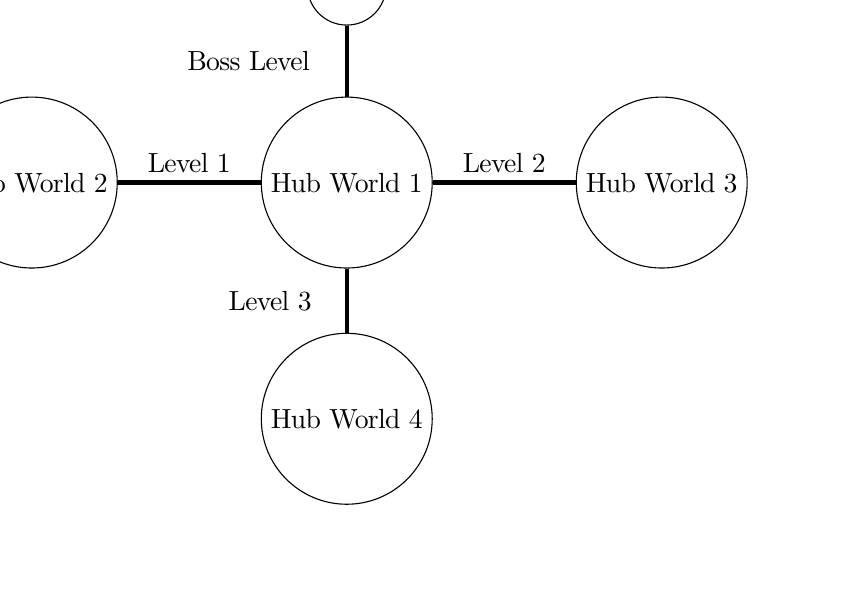
\begin{tikzpicture}
\node[name=Hub-World-2,draw,circle,minimum size=1cm,inner sep=3pt] at (-4,0) {Hub World 2};
\node[name=Hub-World-1,draw,circle,minimum size=1cm,inner sep=3pt] at (0,0) {Hub World 1};
\node[name=Hub-World-3,draw,circle,minimum size=1cm,inner sep=3pt] at (4,0) {Hub World 3};
\node[name=Hub-World-4,draw,circle,minimum size=1cm,inner sep=3pt] at (0,-3) {Hub World 4};
\node[name=Boss,draw,circle,minimum size=1cm,inner sep=-1pt] at (0,2.5) {Boss};

\path [draw] (Hub-World-2) -- node[name=Level-1, midway, above] {Level 1} (Hub-World-1);
\path [draw] (Hub-World-1) -- node[name=Level-2, midway, above] {Level 2} (Hub-World-3);
\path [draw] (Hub-World-1) -- node[name=Level-3, text width=3cm, midway] {Level 3} (Hub-World-4);
\path [draw] (Hub-World-1) -- node[name=Boss-Level, text width=4.05cm, midway] {Boss Level} (Boss);

\draw[ultra thick] (Hub-World-2) -- (Hub-World-1);
\draw[ultra thick] (Hub-World-1) -- (Hub-World-3);
\draw[ultra thick] (Hub-World-1) -- (Hub-World-4);
\draw[ultra thick] (Hub-World-1) -- (Boss);
\end{tikzpicture}
\end{center}
\newpage

\section{Universal Game Mechanics}
\noindent Not Bold = Mechanics \newline
\textbf{Bold = Hazards}
\begin{multicols}{2}
\begin{itemize}[noitemsep]
\item Checkpoints
\item Ladders
\item Reach Stalker
\item \textbf{Straddle Carrier}
\item \textbf{Ramming Cars}
\item Rails
\item Breakable Blocks
\item \textbf{Acid}
\item Puzzle Objects
\item \textbf{Water}
\item Fruits
\item Snow
\item Slippery Ice
\item \textbf{Icicles}
\item \textbf{Electrocuted Rollercoaster Rails}
\item \textbf{Plant Platforms}
\item \textbf{Spikes}
\item \textbf{Searchlights}
\item Teleporters
\item Jump Pads
\item \textbf{Wormholes}
\item Air Gust
\item Movement Accelerator by Wind
\item \textbf{Thunderstorms}
\end{itemize}
\end{multicols}
\newpage
\section{Game Levels}
\centerline{\large \textbf{LEGEND}}
\begin{description}[align=right,labelwidth=3cm,noitemsep]
\item [Fight Level:] A stage where the player mainly fights enemies
\item [Platform Level:] A stage where the player jumps, swings, bounces, or perform any other body movement through obstacles
\begin{description}[align=right,labelwidth=2.5cm,noitemsep,nosep]
\item [Speed Level:] A stage where the player uses a vehicle and requires speed to pass the level
\item [Dig Level:] A stage where the player has to dig underground
\end{description}
\item [Puzzle Level:] A stage where the player has to solve a series of puzzles to pass the level
\item [Stealth Level:] A stage where the player has to hide from enemies to pass the level
\item [Combo Level:] the boss stage that mixes up all (three) of the types of stages (given in the World)
\end{description}
\subsection{Route 6}
\begin{figure}[h]
    \centering
    \begin{multicols}{2}
        \includegraphics[width=3in]{USA}
        \includegraphics[width=3.09in]{US-6}
    \end{multicols}
    \caption{USA (right picture source: Wikipedia)}
\end{figure}
\begin{addmargin}[5mm]{0em}
\textbf{Description:} This is a man-made urban city built around a large metropolis arranged with streets, roads and construction zones. \\ %The people there are . \\
\noindent \textbf{Brands:} Autozone $\bullet$ Advance Auto Parts $\bullet$ Valvoline $\bullet$ Macco $\bullet$ Sunoco \\
\noindent \textbf{Story:} Our hero sets off walking around the metropolis in search for a secret while the gangsters are bringing their hot goods to their leader. For faster time, they drive through the highways, which prohibits pedestrians to enter the highways. In order to do this he has to figure out a way to make a car fast with a stipend provided.
\end{addmargin}
*\textit{Note: This World will be used in the demo for a test run.}
\begin{multicols}{2}
\noindent \textbf{Level 1:} Ivory Road \newline
\indent \textbf{Type:} Fight
\begin{addmargin}[5mm]{0em}
\textbf{Progression:} The player will learn how to fight against some of the thieves. And going this way will lead to another store to buy other parts needed to make the car. %In this World, not only will the player learn how to play the game, but will also buy parts to create a vehicle (i.e., motorcycle, car) used for a few levels that involve riding on highways.
\end{addmargin}
\indent\indent \textbf{Est. play time:} 10 minutes
\begin{addmargin}[5mm]{0em}
\textbf{Color map:} Black (asphalt road) $\bullet$ White (lane markings) $\bullet$ Yellow (lane markings) $\bullet$ Blue (clouds) $\bullet$ Cyan (sky) $\bullet$ Tan (buildings)
\end{addmargin}
\begin{addmargin}[5mm]{0em}
\textbf{Enemies:} Thieves
\end{addmargin}
\begin{addmargin}[5mm]{0em}
\textbf{Mechanics:} Checkpoints $\bullet$ Ladders
\end{addmargin}
\begin{comment}
\begin{addmargin}[5mm]{0em}
\textbf{Hazards:} 
\end{addmargin}
\begin{addmargin}[5mm]{0em}
\textbf{Power-Ups:} $\bullet$
\end{addmargin}
\indent\indent \textbf{Economy:}  \newline
\end{comment}
%\indent \textbf{Music Track:} 
%\includegraphics[width=2.28in]{} \newline
%\\
\columnbreak
\noindent \textbf{Level 2:} Cobalt Thruway \newline
\indent \textbf{Type:} Platform
\begin{addmargin}[5mm]{0em}
\textbf{Progression:} The player will learn how to jump on certain platforms and avoid hazards. This way will lead the player to ask someone to make the car for them before the gangsters leave the city.
\end{addmargin}
\indent\indent \textbf{Est. play time:} 10 minutes
\begin{addmargin}[5mm]{0em}
\textbf{Color map:} Black (asphalt roads) $\bullet$ White (lane markings, rails) $\bullet$ Yellow (lane markings, construction vehicles) $\bullet$ Blue (clouds) $\bullet$ Cyan (sky) $\bullet$ Tan (buildings) $\bullet$ Red (buildings, rails) $\bullet$ Gray (construction vehicles, steel floor plates)
\end{addmargin}
\begin{addmargin}[5mm]{0em}
\textbf{Enemies:} Thieves $\bullet$ Military Guards
\end{addmargin}
\begin{addmargin}[5mm]{0em}
\textbf{Mechanics:} Checkpoints $\bullet$ Ladders $\bullet$ Reach Stalker% $\bullet$
\end{addmargin}
\begin{addmargin}[5mm]{0em}
\textbf{Hazards:} Straddle Carrier $\bullet$ Ramming Cars
\end{addmargin}
%\begin{addmargin}[5mm]{0em}
%\textbf{Power-Ups:} $\bullet$
%\end{addmargin}
%\indent\indent \textbf{Economy:}  \newline
%\indent \textbf{Music Track:} 
%\includegraphics[width=2.28in]{} \newline
\end{multicols}
\newpage
\begin{multicols}{2}
\noindent \textbf{Level 3:} Scarlet Bridge \newline
\indent \textbf{Type:} Speed
\begin{addmargin}[5mm]{0em}
\textbf{Progression:} The player will learn how to drive a vehicle. Now that the player's vehicle is built, it has a little gas, but needs more. This way will lead the player to grab some gasoline and oil before catching up to the target.
\end{addmargin}
\indent\indent \textbf{Est. play time:} 10 minutes
\begin{addmargin}[5mm]{0em}
\textbf{Color map:} Black (asphalt roads) $\bullet$ White (lane markings, rails) $\bullet$ Yellow (lane markings, construction vehicles) $\bullet$ Blue (clouds) $\bullet$ Red (buildings, rails, bridge) $\bullet$ Cyan (sky) $\bullet$ Tan (buildings) $\bullet$ Gray (construction vehicles, steel floor plates) $\bullet$ Green (chevron arrows)
\end{addmargin}
\begin{addmargin}[5mm]{0em}
\textbf{Enemies:} Thieves' Vehicles
\end{addmargin}
\begin{addmargin}[5mm]{0em}
\textbf{Mechanics:} Checkpoints
\end{addmargin}
\begin{addmargin}[5mm]{0em}
\textbf{Hazards:} Ramming Cars
\end{addmargin}
\begin{comment}
\begin{addmargin}[5mm]{0em}
\textbf{Power-Ups:} $\bullet$
\end{addmargin}
\indent\indent \textbf{Economy:}  \newline
\end{comment}
%\indent \textbf{Music Track:} 
%\includegraphics[width=2.28in]{} \newline
%\\
\columnbreak
\noindent \textbf{Level 4:} Steel Convoy \newline
\indent \textbf{Type:} Combo
%\begin{addmargin}[5mm]{0em}
%\textbf{Story:} 
%\end{addmargin}
\begin{addmargin}[5mm]{0em}
\textbf{Progression:} This is where all the types of levels in this World combining into one are introduced. This is the way to reach to the boss of this World. Should the player succeed, the player goes to another World.
\end{addmargin}
\indent\indent \textbf{Est. play time:} 15 minutes
\begin{addmargin}[5mm]{0em}
\textbf{Color map:} Black (asphalt roads) $\bullet$ White (lane markings) $\bullet$ Blue (clouds) $\bullet$ Red (buildings, rails) $\bullet$ Cyan (sky) $\bullet$ Tan (buildings) $\bullet$ Gray (steel floor plates)
\end{addmargin}
\begin{addmargin}[5mm]{0em}
\textbf{Enemies:} Gangsters
\end{addmargin}
\begin{addmargin}[5mm]{0em}
\textbf{Boss:} TBA % (See page \pageref{MechaSally})
\end{addmargin}
\begin{addmargin}[5mm]{0em}
\textbf{Mechanics:} Checkpoints $\bullet$ Ladders $\bullet$ Reach Stalker %$\bullet$ 
\end{addmargin}
\begin{addmargin}[5mm]{0em}
\textbf{Hazards:} Straddle Carrier $\bullet$ Ramming Cars
\end{addmargin}
\begin{comment}
\begin{addmargin}[5mm]{0em}
\textbf{Power-Ups:} $\bullet$
\end{addmargin}
\indent\indent \textbf{Economy:}  \newline
\end{comment}
%\indent \textbf{Music Track:} 
%\includegraphics[width=2.28in]{} \newline
\end{multicols}
\newpage

\begin{comment}
\subsection{Candy Country}
\begin{figure}[h]
    \centering
    \textcolor[HTML]{FFFF00}{\EUCountry{132}}
    \caption{Belgium}
\end{figure}
\begin{addmargin}[5mm]{0em}
\textbf{Brands:} Bed, Bath \& Beyond $\bullet$ Crate \& Barrel $\bullet$ Pottery Barn $\bullet$ IT'SUGAR \\
\noindent \textbf{Description:} This is a happy land filled with candies, chocolate, cake and castles.
\end{addmargin}
\begin{multicols}{2}
\noindent \textbf{Level 1:} Cake Desert \newline
\indent \textbf{Type:} Dig
\begin{addmargin}[5mm]{0em}
\textbf{Story:} 
\end{addmargin}
\begin{addmargin}[5mm]{0em}
\textbf{Progression:} In this World, the player will buy tools to dig underground and various locations in the levels and find rare candies that can be sold at any Hub World in this World.
\end{addmargin}
\indent\indent \textbf{Est. play time}
\begin{addmargin}[5mm]{0em}
\textbf{Color map:} $\bullet$
\end{addmargin}
\begin{addmargin}[5mm]{0em}
\textbf{Enemies:} $\bullet$
\end{addmargin}
\begin{addmargin}[5mm]{0em}
\textbf{Mechanics:} Checkpoints $\bullet$ Ladders $\bullet$
\end{addmargin}
\begin{addmargin}[5mm]{0em}
\textbf{Hazards:} 
\end{addmargin}
\begin{addmargin}[5mm]{0em}
\textbf{Power-Ups:} $\bullet$
\end{addmargin}
\indent\indent \textbf{Economy:}  \newline
\indent \textbf{Music Track:} 
%\includegraphics[width=2.28in]{} \newline
\\
\columnbreak
\noindent \textbf{Level 2:} Chocolate Conduit \newline
\indent \textbf{Type:} Speed
\begin{addmargin}[5mm]{0em}
\textbf{Story:} 
\end{addmargin}
\begin{addmargin}[5mm]{0em}
\textbf{Progression:} 
\end{addmargin}
\indent\indent \textbf{Est. play time}
\begin{addmargin}[5mm]{0em}
\textbf{Color map:} $\bullet$
\end{addmargin}
\begin{addmargin}[5mm]{0em}
\textbf{Enemies:} $\bullet$
\end{addmargin}
\begin{addmargin}[5mm]{0em}
\textbf{Mechanics:} Checkpoints $\bullet$ Ladders $\bullet$
\end{addmargin}
\begin{addmargin}[5mm]{0em}
\textbf{Hazards:} 
\end{addmargin}
\begin{addmargin}[5mm]{0em}
\textbf{Power-Ups:} $\bullet$
\end{addmargin}
\indent\indent \textbf{Economy:}  \newline
\indent \textbf{Music Track:} 
%\includegraphics[width=2.28in]{} \newline
\end{multicols}
\newpage
\begin{multicols}{2}
\noindent \textbf{Level 3:} Jelly Jubilee \newline
\indent \textbf{Type:} Platform
\begin{addmargin}[5mm]{0em}
\textbf{Story:} 
\end{addmargin}
\begin{addmargin}[5mm]{0em}
\textbf{Progression:} 
\end{addmargin}
\indent\indent \textbf{Est. play time}
\begin{addmargin}[5mm]{0em}
\textbf{Color map:} $\bullet$
\end{addmargin}
\begin{addmargin}[5mm]{0em}
\textbf{Enemies:} $\bullet$
\end{addmargin}
\begin{addmargin}[5mm]{0em}
\textbf{Mechanics:} Checkpoints $\bullet$ Ladders $\bullet$
\end{addmargin}
\begin{addmargin}[5mm]{0em}
\textbf{Hazards:} Acid $\bullet$ Spikes
\end{addmargin}
\begin{addmargin}[5mm]{0em}
\textbf{Power-Ups:} $\bullet$
\end{addmargin}
\indent\indent \textbf{Economy:}  \newline
\indent \textbf{Music Track:} 
%\includegraphics[width=2.28in]{} \newline
\\
\columnbreak
\noindent \textbf{Level 4:} Soda Springs \newline
\indent \textbf{Type:} Combo
\begin{addmargin}[5mm]{0em}
\textbf{Story:} 
\end{addmargin}
\begin{addmargin}[5mm]{0em}
\textbf{Progression:} 
\end{addmargin}
\indent\indent \textbf{Est. play time}
\begin{addmargin}[5mm]{0em}
\textbf{Color map:} $\bullet$
\end{addmargin}
\begin{addmargin}[5mm]{0em}
\textbf{Enemies:} $\bullet$
\end{addmargin}
\begin{addmargin}[5mm]{0em}
\textbf{Boss:} \\ % (See page \pageref{MechaSally})
\end{addmargin}
\begin{addmargin}[5mm]{0em}
\textbf{Mechanics:} Checkpoints $\bullet$ Ladders $\bullet$
\end{addmargin}
\begin{addmargin}[5mm]{0em}
\textbf{Hazards:} Acid
\end{addmargin}
\begin{addmargin}[5mm]{0em}
\textbf{Power-Ups:} $\bullet$
\end{addmargin}
\indent\indent \textbf{Economy:}  \newline
\indent \textbf{Music Track:} 
%\includegraphics[width=2.28in]{} \newline
\end{multicols}
\newpage

\subsection{Aqua Beach}
\begin{figure}[h]
    \centering
    \textcolor[HTML]{0000FF}{\EUCountry{143}}
    \caption{Greece}
\end{figure}
\begin{addmargin}[5mm]{0em}
\textbf{Brands:} Quiksilver $\bullet$ Billabong \\
\noindent \textbf{Description:} 
\end{addmargin}
\begin{multicols}{2}
\noindent \textbf{Level 1:} Coastal Shore \newline
\indent \textbf{Type:} Fight
\begin{addmargin}[5mm]{0em}
\textbf{Story:} 
\end{addmargin}
\begin{addmargin}[5mm]{0em}
\textbf{Progression:} In this World, the player will buy gear for riding on water.
\end{addmargin}
\indent\indent \textbf{Est. play time}
\begin{addmargin}[5mm]{0em}
\textbf{Color map:} $\bullet$
\end{addmargin}
\begin{addmargin}[5mm]{0em}
\textbf{Enemies:} $\bullet$
\end{addmargin}
\begin{addmargin}[5mm]{0em}
\textbf{Mechanics:} Checkpoints $\bullet$ Ladders $\bullet$
\end{addmargin}
\begin{addmargin}[5mm]{0em}
\textbf{Hazards:} 
\end{addmargin}
\begin{addmargin}[5mm]{0em}
\textbf{Power-Ups:} $\bullet$
\end{addmargin}
\indent\indent \textbf{Economy:}  \newline
\indent \textbf{Music Track:} 
%\includegraphics[width=2.28in]{} \newline
\\
\columnbreak
\noindent \textbf{Level 2:} Fruity Jungle \newline
\indent \textbf{Type:} Puzzle
\begin{addmargin}[5mm]{0em}
\textbf{Story:} 
\end{addmargin}
\begin{addmargin}[5mm]{0em}
\textbf{Progression:} 
\end{addmargin}
\indent\indent \textbf{Est. play time}
\begin{addmargin}[5mm]{0em}
\textbf{Color map:} $\bullet$
\end{addmargin}
\begin{addmargin}[5mm]{0em}
\textbf{Enemies:} $\bullet$
\end{addmargin}
\begin{addmargin}[5mm]{0em}
\textbf{Mechanics:} Checkpoints $\bullet$ Ladders $\bullet$ Puzzle Objects
\end{addmargin}
\begin{addmargin}[5mm]{0em}
\textbf{Hazards:} Fruits
\end{addmargin}
\begin{addmargin}[5mm]{0em}
\textbf{Power-Ups:} $\bullet$
\end{addmargin}
\indent\indent \textbf{Economy:}  \newline
\indent \textbf{Music Track:} 
%\includegraphics[width=2.28in]{} \newline
\end{multicols}
\newpage
\begin{multicols}{2}
\noindent \textbf{Level 3:} Tubular Aquarium \newline
\indent \textbf{Type:} Speed
\begin{addmargin}[5mm]{0em}
\textbf{Story:} 
\end{addmargin}
\begin{addmargin}[5mm]{0em}
\textbf{Progression:} 
\end{addmargin}
\indent\indent \textbf{Est. play time}
\begin{addmargin}[5mm]{0em}
\textbf{Color map:} $\bullet$
\end{addmargin}
\begin{addmargin}[5mm]{0em}
\textbf{Enemies:} $\bullet$
\end{addmargin}
\begin{addmargin}[5mm]{0em}
\textbf{Mechanics:} Checkpoints $\bullet$ Ladders $\bullet$ Rails
\end{addmargin}
\begin{addmargin}[5mm]{0em}
\textbf{Hazards:} Water
\end{addmargin}
\begin{addmargin}[5mm]{0em}
\textbf{Power-Ups:} $\bullet$
\end{addmargin}
\indent\indent \textbf{Economy:}  \newline
\indent \textbf{Music Track:} 
%\includegraphics[width=2.28in]{} \newline
\\
\columnbreak
\noindent \textbf{Level 4:} Cerulean Harbor \newline
\indent \textbf{Type:} Combo
\begin{addmargin}[5mm]{0em}
\textbf{Story:} 
\end{addmargin}
\begin{addmargin}[5mm]{0em}
\textbf{Progression:} 
\end{addmargin}
\indent\indent \textbf{Est. play time}
\begin{addmargin}[5mm]{0em}
\textbf{Color map:} $\bullet$
\end{addmargin}
\begin{addmargin}[5mm]{0em}
\textbf{Enemies:} $\bullet$
\end{addmargin}
\begin{addmargin}[5mm]{0em}
\textbf{Boss:} \\ % (See page \pageref{MechaSally})
\end{addmargin}
\begin{addmargin}[5mm]{0em}
\textbf{Mechanics:} Checkpoints $\bullet$ Ladders $\bullet$
\end{addmargin}
\begin{addmargin}[5mm]{0em}
\textbf{Hazards:} 
\end{addmargin}
\begin{addmargin}[5mm]{0em}
\textbf{Power-Ups:} $\bullet$
\end{addmargin}
\indent\indent \textbf{Economy:}  \newline
\indent \textbf{Music Track:} 
%\includegraphics[width=2.28in]{} \newline
\end{multicols}
\newpage

\subsection{Winter Paradise}
\begin{figure}[h]
    \centering
    \includegraphics[width=4in]{Russia}
    \caption{Russia}
\end{figure}
\begin{addmargin}[5mm]{0em}
\textbf{Brands:} The North Face $\bullet$ Columbia $\bullet$ Timberland $\bullet$ Spyder \\
\noindent \textbf{Description:} 
\end{addmargin}
\begin{multicols}{2}
\noindent \textbf{Level 1:} Frosty Mountains \newline
\indent \textbf{Type:} Dig
\begin{addmargin}[5mm]{0em}
\textbf{Story:} 
\end{addmargin}
\begin{addmargin}[5mm]{0em}
\textbf{Progression:} In this World, the player will buy gear for staying warm and riding on ice.
\end{addmargin}
\indent\indent \textbf{Est. play time}
\begin{addmargin}[5mm]{0em}
\textbf{Color map:} $\bullet$
\end{addmargin}
\begin{addmargin}[5mm]{0em}
\textbf{Enemies:} $\bullet$
\end{addmargin}
\begin{addmargin}[5mm]{0em}
\textbf{Mechanics:} Checkpoints $\bullet$ Ladders $\bullet$ Snow
\end{addmargin}
\begin{addmargin}[5mm]{0em}
\textbf{Hazards:} Icicles
\end{addmargin}
\begin{addmargin}[5mm]{0em}
\textbf{Power-Ups:} $\bullet$
\end{addmargin}
\indent\indent \textbf{Economy:}  \newline
\indent \textbf{Music Track:} 
%\includegraphics[width=2.28in]{} \newline
\\
\columnbreak
\noindent \textbf{Level 2:} Snowy Village \newline
\indent \textbf{Type:} Puzzle
\begin{addmargin}[5mm]{0em}
\textbf{Story:} 
\end{addmargin}
\begin{addmargin}[5mm]{0em}
\textbf{Progression:} 
\end{addmargin}
\indent\indent \textbf{Est. play time}
\begin{addmargin}[5mm]{0em}
\textbf{Color map:} $\bullet$
\end{addmargin}
\begin{addmargin}[5mm]{0em}
\textbf{Enemies:} $\bullet$
\end{addmargin}
\begin{addmargin}[5mm]{0em}
\textbf{Mechanics:} Checkpoints $\bullet$ Ladders $\bullet$ Snow
\end{addmargin}
\begin{addmargin}[5mm]{0em}
\textbf{Hazards:} 
\end{addmargin}
\begin{addmargin}[5mm]{0em}
\textbf{Power-Ups:} $\bullet$
\end{addmargin}
\indent\indent \textbf{Economy:}  \newline
\indent \textbf{Music Track:} 
%\includegraphics[width=2.28in]{} \newline
\end{multicols}
\newpage
\begin{multicols}{2}
\noindent \textbf{Level 3:} Polar Park \newline
\indent \textbf{Type:} Speed
\begin{addmargin}[5mm]{0em}
\textbf{Story:} 
\end{addmargin}
\begin{addmargin}[5mm]{0em}
\textbf{Progression:} 
\end{addmargin}
\indent\indent \textbf{Est. play time}
\begin{addmargin}[5mm]{0em}
\textbf{Color map:} $\bullet$
\end{addmargin}
\begin{addmargin}[5mm]{0em}
\textbf{Enemies:} $\bullet$
\end{addmargin}
\begin{addmargin}[5mm]{0em}
\textbf{Mechanics:} Checkpoints $\bullet$ Ladders $\bullet$ Snow $\bullet$ Slippery Ice $\bullet$ Rails
\end{addmargin}
\begin{addmargin}[5mm]{0em}
\textbf{Hazards:} Electrocuted Rollercoaster Rails $\bullet$ Icicles
\end{addmargin}
\begin{addmargin}[5mm]{0em}
\textbf{Power-Ups:} $\bullet$
\end{addmargin}
\indent\indent \textbf{Economy:}  \newline
\indent \textbf{Music Track:} 
%\includegraphics[width=2.28in]{} \newline
\\
\columnbreak
\noindent \textbf{Level 4:} Chilly Casino \newline
\indent \textbf{Type:} Combo
\begin{addmargin}[5mm]{0em}
\textbf{Story:} 
\end{addmargin}
\begin{addmargin}[5mm]{0em}
\textbf{Progression:} 
\end{addmargin}
\indent\indent \textbf{Est. play time}
\begin{addmargin}[5mm]{0em}
\textbf{Color map:} $\bullet$
\end{addmargin}
\begin{addmargin}[5mm]{0em}
\textbf{Enemies:} $\bullet$
\end{addmargin}
\begin{addmargin}[5mm]{0em}
\textbf{Boss:} \\ % (See page \pageref{MechaSally})
\end{addmargin}
\begin{addmargin}[5mm]{0em}
\textbf{Mechanics:} Checkpoints $\bullet$ Ladders $\bullet$
\end{addmargin}
\begin{addmargin}[5mm]{0em}
\textbf{Hazards:} 
\end{addmargin}
\begin{addmargin}[5mm]{0em}
\textbf{Power-Ups:} $\bullet$
\end{addmargin}
\indent\indent \textbf{Economy:}  \newline
\indent \textbf{Music Track:} 
%\includegraphics[width=2.28in]{} \newline
\end{multicols}
\newpage
%\end{comment}

\subsection{Vernal Forest}
\begin{figure}[h]
    \centering
    \textcolor[HTML]{00FF00}{\EUCountry{147}}
    \caption{Italy}
\end{figure}
\begin{addmargin}[5mm]{0em}
\textbf{Brands:} L.L.Bean $\bullet$ REI $\bullet$ Dick's Sporting Goods \\
\noindent \textbf{Description:} 
\end{addmargin}
\begin{multicols}{2}
\noindent \textbf{Level 1:} Dawn Hill \newline
\indent \textbf{Type:} Platform
\begin{addmargin}[5mm]{0em}
\textbf{Story:} 
\end{addmargin}
\begin{addmargin}[5mm]{0em}
\textbf{Progression:} In this World, the player will buy gear for surviving the outdoors.
\end{addmargin}
\indent\indent \textbf{Est. play time}
\begin{addmargin}[5mm]{0em}
\textbf{Color map:} $\bullet$
\end{addmargin}
\begin{addmargin}[5mm]{0em}
\textbf{Enemies:} $\bullet$
\end{addmargin}
\begin{addmargin}[5mm]{0em}
\textbf{Mechanics:} Checkpoints $\bullet$ Ladders $\bullet$ Rails
\end{addmargin}
\begin{addmargin}[5mm]{0em}
\textbf{Hazards:} Plant Platforms $\bullet$ Spikes
\end{addmargin}
\begin{addmargin}[5mm]{0em}
\textbf{Power-Ups:} $\bullet$
\end{addmargin}
\indent\indent \textbf{Economy:}  \newline
\indent \textbf{Music Track:} 
%\includegraphics[width=2.28in]{} \newline
\\
\columnbreak
\noindent \textbf{Level 2:} Dusk Woods \newline
\indent \textbf{Type:} Fight
\begin{addmargin}[5mm]{0em}
\textbf{Story:} 
\end{addmargin}
\begin{addmargin}[5mm]{0em}
\textbf{Progression:} 
\end{addmargin}
\indent\indent \textbf{Est. play time}
\begin{addmargin}[5mm]{0em}
\textbf{Color map:} $\bullet$
\end{addmargin}
\begin{addmargin}[5mm]{0em}
\textbf{Enemies:} $\bullet$
\end{addmargin}
\begin{addmargin}[5mm]{0em}
\textbf{Mechanics:} Checkpoints $\bullet$ Ladders $\bullet$
\end{addmargin}
\begin{addmargin}[5mm]{0em}
\textbf{Hazards:} 
\end{addmargin}
\begin{addmargin}[5mm]{0em}
\textbf{Power-Ups:} $\bullet$
\end{addmargin}
\indent\indent \textbf{Economy:}  \newline
\indent \textbf{Music Track:} 
%\includegraphics[width=2.28in]{} \newline
\end{multicols}
\newpage
\begin{multicols}{2}
\noindent \textbf{Level 3:} Rainy Cave \newline
\indent \textbf{Type:} Stealth
\begin{addmargin}[5mm]{0em}
\textbf{Story:} 
\end{addmargin}
\begin{addmargin}[5mm]{0em}
\textbf{Progression:} 
\end{addmargin}
\indent\indent \textbf{Est. play time}
\begin{addmargin}[5mm]{0em}
\textbf{Color map:} $\bullet$
\end{addmargin}
\begin{addmargin}[5mm]{0em}
\textbf{Enemies:} $\bullet$
\end{addmargin}
\begin{addmargin}[5mm]{0em}
\textbf{Mechanics:} Checkpoints $\bullet$ Ladders $\bullet$
\end{addmargin}
\begin{addmargin}[5mm]{0em}
\textbf{Hazards:} Searchlights
\end{addmargin}
\begin{addmargin}[5mm]{0em}
\textbf{Power-Ups:} $\bullet$
\end{addmargin}
\indent\indent \textbf{Economy:}  \newline
\indent \textbf{Music Track:} 
%\includegraphics[width=2.28in]{} \newline
\\
\columnbreak
\noindent \textbf{Level 4:} Abandoned Castle \newline
\indent \textbf{Type:} Combo
\begin{addmargin}[5mm]{0em}
\textbf{Story:} 
\end{addmargin}
\begin{addmargin}[5mm]{0em}
\textbf{Progression:} 
\end{addmargin}
\indent\indent \textbf{Est. play time}
\begin{addmargin}[5mm]{0em}
\textbf{Color map:} $\bullet$
\end{addmargin}
\begin{addmargin}[5mm]{0em}
\textbf{Enemies:} $\bullet$
\end{addmargin}
\begin{addmargin}[5mm]{0em}
\textbf{Boss:} \\ % (See page \pageref{MechaSally})
\end{addmargin}
\begin{addmargin}[5mm]{0em}
\textbf{Mechanics:} Checkpoints $\bullet$ Ladders $\bullet$ Rails
\end{addmargin}
\begin{addmargin}[5mm]{0em}
\textbf{Hazards:} Plant Platforms $\bullet$ Spikes
\end{addmargin}
\begin{addmargin}[5mm]{0em}
\textbf{Power-Ups:} $\bullet$
\end{addmargin}
\indent\indent \textbf{Economy:}  \newline
\indent \textbf{Music Track:} 
%\includegraphics[width=2.28in]{} \newline
\end{multicols}
\newpage

\begin{comment}
\subsection{Game Network}
\begin{figure}[h]
    \centering
    \includegraphics[height=3.25in]{Japan}
    \caption{Japan}
\end{figure}
\begin{addmargin}[5mm]{0em}
\textbf{Brands:} Brookstone $\bullet$ The Sharper Image $\bullet$ SkyMall \\
\noindent \textbf{Description:} 
\end{addmargin}
\begin{multicols}{2}
\noindent \textbf{Level 1:} Techno District \newline
\indent \textbf{Type:} Puzzle
\begin{addmargin}[5mm]{0em}
\textbf{Story:} 
\end{addmargin}
\begin{addmargin}[5mm]{0em}
\textbf{Progression:} 
\end{addmargin}
\indent\indent \textbf{Est. play time}
\begin{addmargin}[5mm]{0em}
\textbf{Color map:} $\bullet$
\end{addmargin}
\begin{addmargin}[5mm]{0em}
\textbf{Enemies:} $\bullet$
\end{addmargin}
\begin{addmargin}[5mm]{0em}
\textbf{Mechanics:} Checkpoints $\bullet$ Ladders $\bullet$ Teleporters
\end{addmargin}
\begin{addmargin}[5mm]{0em}
\textbf{Hazards:} 
\end{addmargin}
\begin{addmargin}[5mm]{0em}
\textbf{Power-Ups:} $\bullet$
\end{addmargin}
\indent\indent \textbf{Economy:}  \newline
\indent \textbf{Music Track:} 
%\includegraphics[width=2.28in]{} \newline
\\
\columnbreak
\noindent \textbf{Level 2:} Time Rush \newline
\indent \textbf{Type:} Speed
\begin{addmargin}[5mm]{0em}
\textbf{Story:} 
\end{addmargin}
\begin{addmargin}[5mm]{0em}
\textbf{Progression:} 
\end{addmargin}
\indent\indent \textbf{Est. play time}
\begin{addmargin}[5mm]{0em}
\textbf{Color map:} $\bullet$
\end{addmargin}
\begin{addmargin}[5mm]{0em}
\textbf{Enemies:} $\bullet$
\end{addmargin}
\begin{addmargin}[5mm]{0em}
\textbf{Mechanics:} Checkpoints $\bullet$ Ladders $\bullet$ Rails $\bullet$ Teleporters $\bullet$ Jump Pads
\end{addmargin}
\begin{addmargin}[5mm]{0em}
\textbf{Hazards:} Wormholes
\end{addmargin}
\begin{addmargin}[5mm]{0em}
\textbf{Power-Ups:} $\bullet$
\end{addmargin}
\indent\indent \textbf{Economy:}  \newline
\indent \textbf{Music Track:} 
%\includegraphics[width=2.28in]{} \newline
\end{multicols}
\newpage
\begin{multicols}{2}
\noindent \textbf{Level 3:} Hidden Cyberpunk \newline
\indent \textbf{Type:} Stealth
\begin{addmargin}[5mm]{0em}
\textbf{Story:} 
\end{addmargin}
\begin{addmargin}[5mm]{0em}
\textbf{Progression:} 
\end{addmargin}
\indent\indent \textbf{Est. play time}
\begin{addmargin}[5mm]{0em}
\textbf{Color map:} $\bullet$
\end{addmargin}
\begin{addmargin}[5mm]{0em}
\textbf{Enemies:} $\bullet$
\end{addmargin}
\begin{addmargin}[5mm]{0em}
\textbf{Mechanics:} Checkpoints $\bullet$ Ladders $\bullet$ Teleporters
\end{addmargin}
\begin{addmargin}[5mm]{0em}
\textbf{Hazards:} Searchlights
\end{addmargin}
\begin{addmargin}[5mm]{0em}
\textbf{Power-Ups:} $\bullet$
\end{addmargin}
\indent\indent \textbf{Economy:}  \newline
\indent \textbf{Music Track:} 
%\includegraphics[width=2.28in]{} \newline
\\
\columnbreak
\noindent \textbf{Level 4:} Virus Void \newline
\indent \textbf{Type:} Combo
\begin{addmargin}[5mm]{0em}
\textbf{Story:} 
\end{addmargin}
\begin{addmargin}[5mm]{0em}
\textbf{Progression:} 
\end{addmargin}
\indent\indent \textbf{Est. play time}
\begin{addmargin}[5mm]{0em}
\textbf{Color map:} $\bullet$
\end{addmargin}
\begin{addmargin}[5mm]{0em}
\textbf{Enemies:} $\bullet$
\end{addmargin}
\begin{addmargin}[5mm]{0em}
\textbf{Boss:} \\ % (See page \pageref{MechaSally})
\end{addmargin}
\begin{addmargin}[5mm]{0em}
\textbf{Mechanics:} Checkpoints $\bullet$ Ladders $\bullet$
\end{addmargin}
\begin{addmargin}[5mm]{0em}
\textbf{Hazards:} 
\end{addmargin}
\begin{addmargin}[5mm]{0em}
\textbf{Power-Ups:} $\bullet$
\end{addmargin}
\indent\indent \textbf{Economy:}  \newline
\indent \textbf{Music Track:} 
%\includegraphics[width=2.28in]{} \newline
\end{multicols}
\newpage

\subsection{Astral Sky}
\begin{addmargin}[5mm]{0em}
\textbf{Brands:} Samsonite \\
\noindent \textbf{Description:} This is a World high above the skies where ancient ruins and floating platforms are located.
\end{addmargin}
\begin{multicols}{2}
\noindent \textbf{Level 1:} Star Realm \newline
\indent \textbf{Type:} Platform
\begin{addmargin}[5mm]{0em}
\textbf{Story:} 
\end{addmargin}
\begin{addmargin}[5mm]{0em}
\textbf{Progression:} In this World, the player will buy mostly everything combined (from previous levels) including parts for a simple plane, gadgets, and wearable gear for flying through the skies.
\end{addmargin}
\indent\indent \textbf{Est. play time}
\begin{addmargin}[5mm]{0em}
\textbf{Color map:} $\bullet$
\end{addmargin}
\begin{addmargin}[5mm]{0em}
\textbf{Enemies:} $\bullet$
\end{addmargin}
\begin{addmargin}[5mm]{0em}
\textbf{Mechanics:} Checkpoints $\bullet$ Ladders $\bullet$
\end{addmargin}
\begin{addmargin}[5mm]{0em}
\textbf{Hazards:} 
\end{addmargin}
\begin{addmargin}[5mm]{0em}
\textbf{Power-Ups:} $\bullet$
\end{addmargin}
\indent\indent \textbf{Economy:}  \newline
\indent \textbf{Music Track:} 
%\includegraphics[width=2.28in]{} \newline
\\
\columnbreak
\noindent \textbf{Level 2:} Cloud Highland \newline
\indent \textbf{Type:} Speed
\begin{addmargin}[5mm]{0em}
\textbf{Story:} 
\end{addmargin}
\begin{addmargin}[5mm]{0em}
\textbf{Progression:} 
\end{addmargin}
\indent\indent \textbf{Est. play time}
\begin{addmargin}[5mm]{0em}
\textbf{Color map:} $\bullet$
\end{addmargin}
\begin{addmargin}[5mm]{0em}
\textbf{Enemies:} $\bullet$
\end{addmargin}
\begin{addmargin}[5mm]{0em}
\textbf{Mechanics:} Checkpoints $\bullet$ Ladders $\bullet$ Rails  $\bullet$ Jump Pads (Clouds) $\bullet$ Air Gust $\bullet$ Movement Accelerator by Wind
\end{addmargin}
\begin{addmargin}[5mm]{0em}
\textbf{Hazards:} 
\end{addmargin}
\begin{addmargin}[5mm]{0em}
\textbf{Power-Ups:} $\bullet$
\end{addmargin}
\indent\indent \textbf{Economy:}  \newline
\indent \textbf{Music Track:} 
%\includegraphics[width=2.28in]{} \newline
\end{multicols}
\newpage
\begin{multicols}{2}
\noindent \textbf{Level 3:} Wish Garden \newline
\indent \textbf{Type:} Puzzle
\begin{addmargin}[5mm]{0em}
\textbf{Story:} 
\end{addmargin}
\begin{addmargin}[5mm]{0em}
\textbf{Progression:} 
\end{addmargin}
\indent\indent \textbf{Est. play time}
\begin{addmargin}[5mm]{0em}
\textbf{Color map:} $\bullet$
\end{addmargin}
\begin{addmargin}[5mm]{0em}
\textbf{Enemies:} $\bullet$
\end{addmargin}
\begin{addmargin}[5mm]{0em}
\textbf{Mechanics:} Checkpoints $\bullet$ Ladders $\bullet$ Breakable Blocks
\end{addmargin}
\begin{addmargin}[5mm]{0em}
\textbf{Hazards:} 
\end{addmargin}
\begin{addmargin}[5mm]{0em}
\textbf{Power-Ups:} $\bullet$
\end{addmargin}
\indent\indent \textbf{Economy:}  \newline
\indent \textbf{Music Track:} 
%\includegraphics[width=2.28in]{} \newline
\\
\columnbreak
\noindent \textbf{Level 4:} Serpent Jump \newline
\indent \textbf{Type:} Combo
\begin{addmargin}[5mm]{0em}
\textbf{Story:} 
\end{addmargin}
\begin{addmargin}[5mm]{0em}
\textbf{Progression:} 
\end{addmargin}
\indent\indent \textbf{Est. play time}
\begin{addmargin}[5mm]{0em}
\textbf{Color map:} $\bullet$
\end{addmargin}
\begin{addmargin}[5mm]{0em}
\textbf{Enemies:} $\bullet$
\end{addmargin}
\begin{addmargin}[5mm]{0em}
\textbf{Boss:} \\ % (See page \pageref{MechaSally})
\end{addmargin}
\begin{addmargin}[5mm]{0em}
\textbf{Mechanics:} Checkpoints $\bullet$ Ladders $\bullet$
\end{addmargin}
\begin{addmargin}[5mm]{0em}
\textbf{Hazards:} Thunderstorms/Lightning
\end{addmargin}
\begin{addmargin}[5mm]{0em}
\textbf{Power-Ups:} $\bullet$
\end{addmargin}
\indent\indent \textbf{Economy:}  \newline
\indent \textbf{Music Track:} 
%\includegraphics[width=2.28in]{} \newline
\end{multicols}
\newpage

\subsection{Base Code 255}
\begin{addmargin}[5mm]{0em}
\textbf{Story:} 
\end{addmargin}
\begin{addmargin}[5mm]{0em}
\textbf{Progression:} 
\end{addmargin}
\begin{addmargin}[5mm]{0em}
\textbf{Est. play time:} 
\end{addmargin}
\begin{addmargin}[5mm]{0em}
\textbf{Color map:} 
\end{addmargin}
\begin{addmargin}[5mm]{0em}
\textbf{Boss:} % (See page \pageref{MechaSally})
\end{addmargin}
\indent\indent \textbf{Music Track:}  \newline \newline
%\includegraphics[width=2.28in]{} \newline
*\textit{Note: This World was originally called TSX (because of Tesla-Space X) until realizing that the Japanese auto manufacturer Honda made a car model called TSX. So by adding the ASCII numbers from those letters, they all add up to 255.}
\newpage
\end{comment}

%\twocolumn

\begin{comment}
\section{Enemies}

\subsection{General Enemy Rules}
\noindent The behavior of an AI (enemy) act by targeting towards Mega Man if they appear in the screen. \newline \newline
Spawn parameter is when an enemy is defeated and if the player goes back and forth as the screen moves, the enemy spawns if the screen displays the enemy in its original location. \newline \newline
Rewards for defeating enemies include Small Life Energy, Small Weapon Energy, Large Life Energy, Large Weapon Energy, 1-Up, Small Screws, and Large Screws.

\subsection{Level-specific Badniks}
\subsection*{Neo Route 99}
\subsubsection*{}
\begin{addmargin}[5mm]{0em}
%\includegraphics[keyvals]{imagefile}
\textbf{Description: } \newline
\textbf{Movement Patterns: }  \newline
\textbf{Attack Description(s): }  \newline
\begin{addmargin}[5mm]{0em}
\textbf{Attack Damage (Contact):}  \newline
\textbf{Attack Damage (Weapon):} 
\end{addmargin}
\textbf{Damage Description: }  \newline
\begin{addmargin}[5mm]{0em}
\textbf{Health Points:} 
\end{addmargin}
\textbf{Particle Effects: } \newline
\end{addmargin}

\onecolumn
\section{Bosses}
\noindent To make this game different, each boss will have four different levels of attack, like a Super Move in a fighting game. Each time a boss (typically Robot Masters) gets hit 7 health points, a level of attack is added. For example, if a boss has one attack and gets hit once, the boss gets a new attack and can use two attacks to fight the player. For some bosses, a level of attack has increased. For example, if a boss gets hit once, the boss gets a new attack and can no longer use the previous attack that the boss used before. When the boss runs out all 28 health points, the boss dies, letting the player accomplish a level.


\subsection*{} \label{}
\begin{wrapfigure}{r}{0.25\textwidth}
\vspace{-20pt}
\begin{center}
%\includegraphics{}
\end{center}
\vspace{-15pt}
\caption*{\footnotesize Art \& Concept: }
\vspace{-15pt}
\end{wrapfigure}
\indent Designer: Spadyal \newline
\begin{addmargin}[10mm]{0em}

\end{addmargin}
\indent\indent Animation List \newline
\indent\indent Entrance
\begin{addmargin}[15mm]{0em}

\end{addmargin}
\indent\indent Movements \newline
\indent\indent  \newline
\indent Attacks \newline
\indent\indent Level 1:  \newline
\indent\indent\indent  \newline
\indent\indent Level 2: 
\begin{addmargin}[15mm]{0em}

\end{addmargin}
\indent\indent\indent Level 3: 
\begin{addmargin}[15mm]{0em}

\end{addmargin}
\indent\indent\indent Level 4: 
\begin{addmargin}[15mm]{0em}

\end{addmargin}
\indent\indent Projectiles \newline
\indent\indent  \newline
\indent Sound Effects List \newline
\indent\indent  \newline
\newpage

\subsection*{} \label{}
\begin{wrapfigure}{r}{0.25\textwidth}
\vspace{-20pt}
\begin{center}
%\includegraphics{}
\end{center}
\vspace{-15pt}
\caption*{\footnotesize Art \& Concept: }
\vspace{-15pt}
\end{wrapfigure}
\indent Designer: Spadyal \newline
\begin{addmargin}[10mm]{0em}

\end{addmargin}
\indent\indent Animation List \newline
\indent\indent Entrance
\begin{addmargin}[15mm]{0em}

\end{addmargin}
\indent\indent Movements \newline
\indent\indent  \newline
\indent Attacks \newline
\indent\indent Level 1:  \newline
\indent\indent\indent  \newline
\indent\indent Level 2: 
\begin{addmargin}[15mm]{0em}

\end{addmargin}
\indent\indent\indent Level 3: 
\begin{addmargin}[15mm]{0em}

\end{addmargin}
\indent\indent\indent Level 4: 
\begin{addmargin}[15mm]{0em}

\end{addmargin}
\indent\indent Projectiles \newline
\indent\indent  \newline
\indent Sound Effects List \newline
\indent\indent  \newline
\newpage

\subsection*{} \label{}
\begin{wrapfigure}{r}{0.25\textwidth}
\vspace{-20pt}
\begin{center}
%\includegraphics{}
\end{center}
\vspace{-15pt}
\caption*{\footnotesize Art \& Concept: }
\vspace{-15pt}
\end{wrapfigure}
\indent Designer: Spadyal \newline
\begin{addmargin}[10mm]{0em}

\end{addmargin}
\indent\indent Animation List \newline
\indent\indent Entrance
\begin{addmargin}[15mm]{0em}

\end{addmargin}
\indent\indent Movements \newline
\indent\indent  \newline
\indent Attacks \newline
\indent\indent Level 1:  \newline
\indent\indent\indent  \newline
\indent\indent Level 2: 
\begin{addmargin}[15mm]{0em}

\end{addmargin}
\indent\indent\indent Level 3: 
\begin{addmargin}[15mm]{0em}

\end{addmargin}
\indent\indent\indent Level 4: 
\begin{addmargin}[15mm]{0em}

\end{addmargin}
\indent\indent Projectiles \newline
\indent\indent  \newline
\indent Sound Effects List \newline
\indent\indent  \newline
\newpage

\subsection*{} \label{}
\begin{wrapfigure}{r}{0.25\textwidth}
\vspace{-20pt}
\begin{center}
%\includegraphics{}
\end{center}
\vspace{-15pt}
\caption*{\footnotesize Art \& Concept: }
\vspace{-15pt}
\end{wrapfigure}
\indent Designer: Spadyal \newline
\begin{addmargin}[10mm]{0em}

\end{addmargin}
\indent\indent Animation List \newline
\indent\indent Entrance
\begin{addmargin}[15mm]{0em}

\end{addmargin}
\indent\indent Movements \newline
\indent\indent  \newline
\indent Attacks \newline
\indent\indent Level 1:  \newline
\indent\indent\indent  \newline
\indent\indent Level 2: 
\begin{addmargin}[15mm]{0em}

\end{addmargin}
\indent\indent\indent Level 3: 
\begin{addmargin}[15mm]{0em}

\end{addmargin}
\indent\indent\indent Level 4: 
\begin{addmargin}[15mm]{0em}

\end{addmargin}
\indent\indent Projectiles \newline
\indent\indent  \newline
\indent Sound Effects List \newline
\indent\indent  \newline
\newpage

\subsection*{} \label{}
\begin{wrapfigure}{r}{0.25\textwidth}
\vspace{-20pt}
\begin{center}
%\includegraphics{}
\end{center}
\vspace{-15pt}
\caption*{\footnotesize Art \& Concept: }
\vspace{-15pt}
\end{wrapfigure}
\indent Designer: Spadyal \newline
\begin{addmargin}[10mm]{0em}

\end{addmargin}
\indent\indent Animation List \newline
\indent\indent Entrance
\begin{addmargin}[15mm]{0em}

\end{addmargin}
\indent\indent Movements \newline
\indent\indent  \newline
\indent Attacks \newline
\indent\indent Level 1:  \newline
\indent\indent\indent  \newline
\indent\indent Level 2: 
\begin{addmargin}[15mm]{0em}

\end{addmargin}
\indent\indent\indent Level 3: 
\begin{addmargin}[15mm]{0em}

\end{addmargin}
\indent\indent\indent Level 4: 
\begin{addmargin}[15mm]{0em}

\end{addmargin}
\indent\indent Projectiles \newline
\indent\indent  \newline
\indent Sound Effects List \newline
\indent\indent  \newline
\newpage

\subsection*{} \label{}
\begin{wrapfigure}{r}{0.25\textwidth}
\vspace{-20pt}
\begin{center}
%\includegraphics{}
\end{center}
\vspace{-15pt}
\caption*{\footnotesize Art \& Concept: }
\vspace{-15pt}
\end{wrapfigure}
\indent Designer: Spadyal \newline
\begin{addmargin}[10mm]{0em}

\end{addmargin}
\indent\indent Animation List \newline
\indent\indent Entrance
\begin{addmargin}[15mm]{0em}

\end{addmargin}
\indent\indent Movements \newline
\indent\indent  \newline
\indent Attacks \newline
\indent\indent Level 1:  \newline
\indent\indent\indent  \newline
\indent\indent Level 2: 
\begin{addmargin}[15mm]{0em}

\end{addmargin}
\indent\indent\indent Level 3: 
\begin{addmargin}[15mm]{0em}

\end{addmargin}
\indent\indent\indent Level 4: 
\begin{addmargin}[15mm]{0em}

\end{addmargin}
\indent\indent Projectiles \newline
\indent\indent  \newline
\indent Sound Effects List \newline
\indent\indent  \newline
\newpage

\subsection*{} \label{}
\begin{wrapfigure}{r}{0.25\textwidth}
\vspace{-20pt}
\begin{center}
%\includegraphics{}
\end{center}
\vspace{-15pt}
\caption*{\footnotesize Art \& Concept: }
\vspace{-15pt}
\end{wrapfigure}
\indent Designer: Spadyal \newline
\begin{addmargin}[10mm]{0em}

\end{addmargin}
\indent\indent Animation List \newline
\indent\indent Entrance
\begin{addmargin}[15mm]{0em}

\end{addmargin}
\indent\indent Movements \newline
\indent\indent  \newline
\indent Attacks \newline
\indent\indent Level 1:  \newline
\indent\indent\indent  \newline
\indent\indent Level 2: 
\begin{addmargin}[15mm]{0em}

\end{addmargin}
\indent\indent\indent Level 3: 
\begin{addmargin}[15mm]{0em}

\end{addmargin}
\indent\indent\indent Level 4: 
\begin{addmargin}[15mm]{0em}

\end{addmargin}
\indent\indent Projectiles \newline
\indent\indent  \newline
\indent Sound Effects List \newline
\indent\indent  \newline
\newpage

\subsection*{} \label{}
\begin{wrapfigure}{r}{0.25\textwidth}
\vspace{-20pt}
\begin{center}
%\includegraphics{}
\end{center}
\vspace{-15pt}
\caption*{\footnotesize Art \& Concept: }
\vspace{-15pt}
\end{wrapfigure}
\indent Designer: Spadyal \newline
\begin{addmargin}[10mm]{0em}

\end{addmargin}
\indent\indent Animation List \newline
\indent\indent Entrance
\begin{addmargin}[15mm]{0em}

\end{addmargin}
\indent\indent Movements \newline
\indent\indent  \newline
\indent Attacks \newline
\indent\indent Level 1:  \newline
\indent\indent\indent  \newline
\indent\indent Level 2: 
\begin{addmargin}[15mm]{0em}

\end{addmargin}
\indent\indent\indent Level 3: 
\begin{addmargin}[15mm]{0em}

\end{addmargin}
\indent\indent\indent Level 4: 
\begin{addmargin}[15mm]{0em}

\end{addmargin}
\indent\indent Projectiles \newline
\indent\indent  \newline
\indent Sound Effects List \newline
\indent\indent  \newline
\newpage

\section{NPCs}

\newpage

\end{comment}

\section{Marketing Idea}

%\noindent In order to use a brand name into the game, we would need to contact a manufacturer and use their name---and probably the logo---and pay to the game developer around \$10. Each game downloaded and played, by a database where when the user begins to play the game, they will post a user ID with a few parameters, such as name. That is, the player will make a view every time the player plays the game, even after quitting the game. This play will be called an ``Ignition.'' Like an impression, the number of \_ of a particular brand advertised is determined by the number of times the game is loaded and added into an attribute into the database called ``View Count.'' \newline \newline
%Just for a test run for a demo, the manufacturer

\twocolumn

\begin{comment}
\section{Music}
\tablehead{
}

\tablelasttail{
\\
}

\noindent \textbf{Awakening:} The music genres are Trance and Progressive House, which both those genres give a cheerful tone. \newline
\begin{supertabular}{r|l}
&  \\ \hline
&  \\ \hline
&  \\ \hline
&  \\ \hline
&  \\ \hline
& 
\end{supertabular}
\onecolumn

\section{Screens}

\subsection{Credits}
\begin{multicols}{2}

\end{multicols}
\newpage

\subsection{Bonus Material}

\onecolumn

\subsection{Special Features}
\subsubsection{Fun Facts}

\subsubsection*{Time To Make}

\subsubsection*{Development Story}

\subsubsection*{Acknowledgements}

\newpage

\section{Appendixes}

\subsection{Sound Effects List}

\end{comment}
\end{document}